\documentclass{article}
\usepackage[utf8]{inputenc}
\usepackage[T1]{fontenc}
\usepackage[MeX]{polski}
\usepackage{graphicx}
\usepackage[outdir=./]{epstopdf}
\usepackage{listings}

\title{%
	Implementacja i przetestowanie algorytmów \\
	dokładnych i przybliżonych \\
	dla problemów szeregowania zadań \\
	kompatybilnych na maszynach jednorodnych}
	

\author{Tomasz Wesołowski}
\date{2019}
 
\begin{document}
 
\maketitle
 
\tableofcontents
 
\section{Problem szeregowania zadań}

Szeregowanie zadań kompatybilnych na maszynach jednorodnych.

\subsection{Przykłady zastosowań}

\paragraph{} Wyobraźmy sobie, że prowadzimy firmę transportową zajmującą się przewozem zwierząt. Danego dnia mamy do przewiezienia $n$ zwierząt, z czego każde jest mniej lub bardziej problematyczne, a co za tym idzie koszt jego przewiezienia jest droższy. Dodatkowo nie wszystkie zwierzęta można przewozić ze sobą, ponieważ, na przykład, kota nie można przewozić razem z psem, myszy ze słoniem, a węża z chomikiem. 
Wszyscy nasi pracownicy otrzymują takie samo wynagrodzenie, płacone od godziny, ale różnią się między sobą umiejętnościami i sprawnością, więc wykonują swoją pracę w różnym tempie. W jaki sposób możemy zminimalizować nasz koszt, przydzielając najbardziej sprawnych pracowników do zwierząt, których transport będzie kosztował najwięcej? W tym przykładzie wierzchołkami są zwierzęta z wagami odzwierciedlającymi koszty transportu. Krawędzie w grafie odpowiadajć zwierzętom, które nie mogą być w jednym transporcie. Kolorowaniem takiego grafu będzie przyporządkowanie pracowników.

Innym przykładem będzie organizacja warsztatów na dużej, międzynajodowej konferencji. W ramach warsztatów mamy za zadanie zorganizować $n$ szkoleń, na każde zapisało się (i opłaciło udział) już wielu uczestników. Godziny szkoleń mogą się na siebie nakładać. Im więcej osób zapisało się na warsztat, tym koszt poprowadzenia takiego warszatu jest droższy, ponieważ trzeba zapewnić odpowiednie akcesoria do wykonania ćwiczeń oraz zapewnić odpowiednio dużą salę, co wiąże się z odpowiednio wysokim kosztem. Mamy do dyspozycji kilka sal, każda o innym koszcie (każda jest w stanie pomieścić uczestników największego szkolenia). Jak rozmieścić szkolenia w salach, tak by zminimalizować koszt?

\section{Algorytmy kolorowania grafów ważonych}

Aby przejść do rozwiązywania problemu kosztowego kolorowania grafów ważonych musimy zacząć od kilku definicji formalnych. 

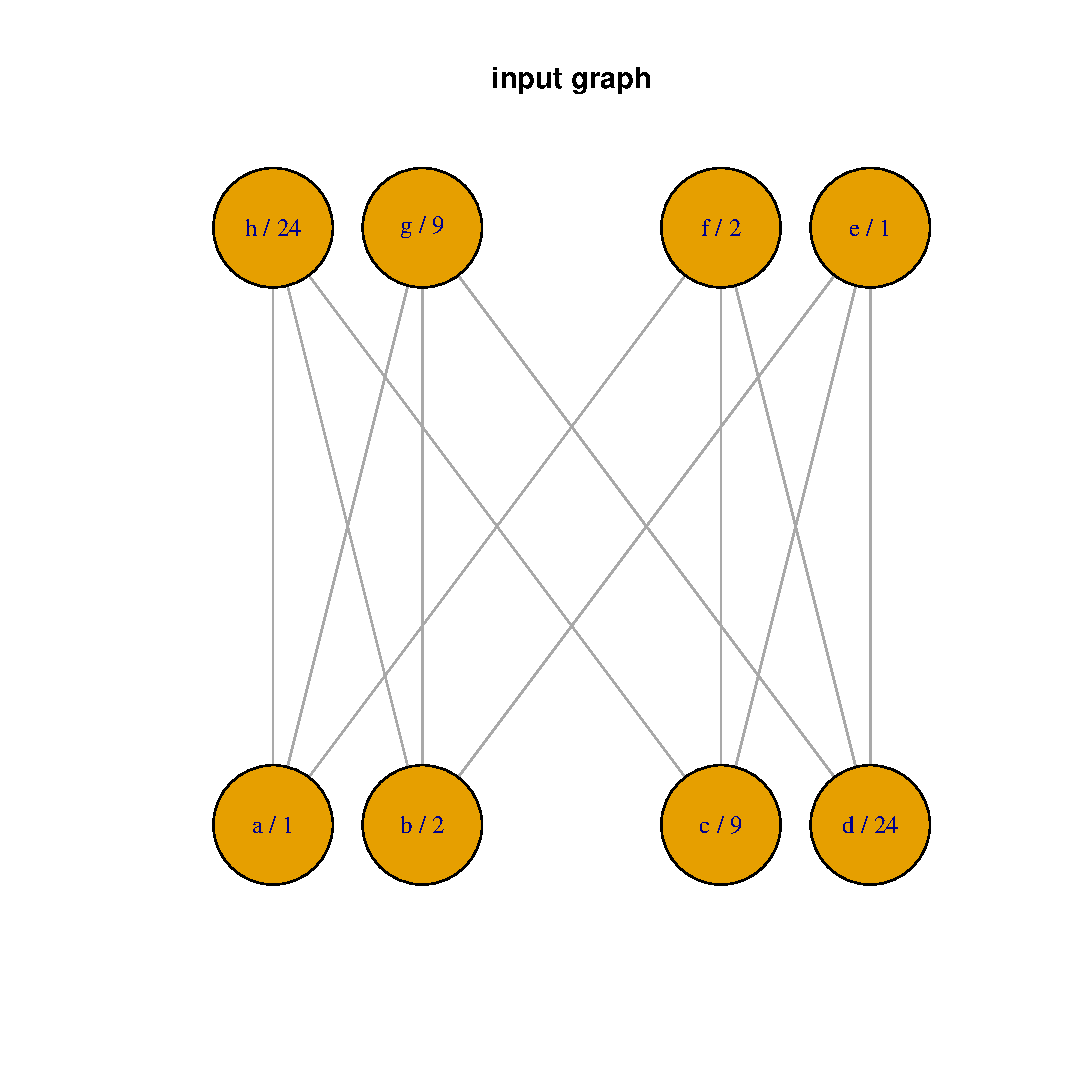
\includegraphics[scale=0.6]{graphs/reference_graph.eps}

I tak, mając graf ważony $G_w = (V,E,w)$, gdzie $V$ to zbiór wierzchołków, $E$ to zbiór krawędzi, natomiast $w$ to wagi wierzchołków takie, że  $w:V \rightarrow R_+$ oraz palete (zestaw) kolorów $C = (c_1, c_2, ..)$ taką że $\forall c_i \in N_+$ staramy się znaleźć takie przyporządkowanie kolorów do wierzchołków, by zminimalizować sumę iloczynów wag w grafie $\sum w_i * c_i = min$ oraz by żadne dwa wierzchołki mające wspólną krawędź nie miały tego samego koloru. Innymi słowy szukamy optymalnego, poprawnego kolorowania grafu.

Problem kosztowego kolorowania grafów ważonych jest problemem optymalizacyjnym, NP-trudnym. Z racji na złożoność problemu, w tej pracy zajmiemy się tylko grafami dwudzielnymi oraz weźmiemy pod uwagę tylko palety składające się z co najwyżej 4 kolorów.

\subsection{Algorytm przybliżony}

\subsubsection*{3-pseudo kolorowanie}

K-pseudokolorowaniem grafu nazywamy każde poprawne kolorowanie $k-1$ kolorami lub kolorowanie $k$ kolorami takie, że wierzchołki pokolorowane ostatnim kolorem mogą nie być niezależne, tzn. wierzchołki pokolorowane ostatnim kolorem mogą być połączone krawędziami między sobą. 

Minimalne k-pseudokolorowanie polega na takim dobraniu kolorów, by spełnione były warunki k-pseudokolorowania oraz suma iloczynów wag wierzchołków i wag kolorów była jak najmniejsza.

Algorytm polega na zbudowaniu grafu skierowanego na podstawie grafu wejściowego i wyliczeniu przecięcia S-T. W ten sposób utworzone zbiory wierzchołków, po drobnych przekształceniach, definiują 3 kolory jakimi należy pokolorować graf by otrzymać 3-pseudokolorowanie. Algorytm został znakomicie opisany w \cite{kubale-pikies19}.

\subsubsection*{27/26-przybliżony}

Algorytm 27/26-przybliżony działa w czasie $O(nm)$, ale nie gwarantuje nam znalezienia optymalnego rozwiązania. Mamy jednak pewność, że znalezione rozwiązanie nie będzie gorsze niż 27/26 rozwiązania optymalnego. 

Pierwszym krokiem jest wyznaczenie zbiorów kolorów $V1$, $V2$ oraz $V3$ poprzez algorytm minimalnego 3-pseudokolorowania. Następnie kolorujemy graf optymalnie kolorami $C1$ oraz $C2$ i obliczamy sumę kolorowania, oznaczamy ją $S1$. 

Kolejnym krokiem jest pokolorowanie kolorem $C1$ wierzchołków $V1$ które otrzymaliśmy z 3-pseudokolorowania, a pozostałą część wierzchołków kolorujemy optymalnie kolorami $C2$ oraz $C3$ i takie kolorowanie oznaczamy jako $S2$.

Następnie kolorujemy $V1$ kolorem $C1$, $V2$ kolorem $C2$, a pozostałe wierzchołki kolorujemy optymalnie $C3$ oraz $C4$ i takie pokolorowanie oznaczamy jako $S3$.

Najlepsze z pokolorowań $S1$, $S2$ oraz $S3$ (kryterium jest minimum sumy kolorowania) jest naszym rozwiązaniem. Co więcej, jest rozwiązaniem nie gorszym niż 27/26 rozwiązania optymalnego jak zostało dowiedzione w \cite{kubale-pikies19}.

\subsubsection*{Wstępna selekcja grafów łatwych}

Grafy banalne do wyliczenia optymalnego wyniku możemy łatwo zidentyfikować już na początku algorytmu. W takich przypadkach optymalne rozwiązanie uzyskujemy już w pierwszym kroku algoytmu imamy pewność że kolejne kroki nie polepszą wyniku, więc algorytm można przerwać wcześniej.

By to osiągnąć, po obliczeniu optymalnego kolorowania dwoma kolorami należy obliczyć najcięższy zbiór niezależny. Jeśli suma wag wierzchołków wyznaczonych przez ten zbiór, oraz suma wag wyznaczonych przez któryś z kolorów z dwukolorowania są sobie równe, oznacza to że osiągneliśmy wynik optymalny.

\subsection{Algorytm optymalny}

\paragraph{} Algorytm optymalny opiera się na metodzie siłowej, gdzie generujemy wszystkie możliwe sekwencje kolorów dla danego grafu. Ilość wszystkich kombinacji wynosi $n^k$, gdzie $n$ to ilość wierzchołków grafu, a $k$ to ilość różnych kolorów - w naszym przypadku 4. Sposób przypisania kolorów do wierzchołków w danej sekwencji definiuje wzór $c = (x / k^{i-1}) \bmod k$, gdzie $c$ to index koloru, $i$ to index wierzchołka w grafie, $x$ to numer danej sekwencji a $k$ ilość dostępnych kolorów w palecie. 

Dla każdej wygenerowanej kombinacji musimy wykonać dwa obliczenia. Należy zweryfikować, czy dana kombinacja jest poprawnym kolorowaniem, oraz obliczyć sumę kolorowania, by można było wybrać najlepszy wynik.

Sprawdzenie, czy kolorowanie jest poprawne czy nie jest banalne i polega na odwiedzeniu wszystkich wierzchołków w dowolnej kolejności oraz sprawdzeniu, czy dany wierzchołek nie ma sąsiada w tym samym kolorze co on. W celu optymalizacji, można sprawdzać wierzchołki w kolejności malejącej biorąc pod uwagę stopień wierzchołka.

\subsubsection*{Zrównoleglenie}

\paragraph{} Algorytm możemy podzielić na sekwencje trzech kroków, W pierwszym kroku generujemy wszystkie możliwe kombinacje kolorów, następnie wykonujemy obliczenia dla każdej z kombinacji a na końcu musimy wybrać najlepszą wynik (kombinacje, dla której suma kolorowania jest najmniejsza).

Algorytm jest stosunkowo łatwy do zrównoleglenia, ponieważ pierwsza i ostatnia faza są proste obliczeniowo, natomiast w przypadku fazy środkowej (najbardziej wymagającej obliczeniowo) obliczenia możemy wykonywać równolegle, każdą z kombinacji liczyć niezależnie.

\subsubsection*{Odrzucanie rozwiązań które dają sumę większą zadanej wartości}

\paragraph{} Na każdej wygenerowanej kombincaji kolorów musimy wykonać dwa obliczenia: policzenie sumy kolorowania oraz zweryfikowanie, czy otrzymana kombinacja kolorów jest kolorowaniem poprawnym. Możemy zredukować ilość obliczeń, najpierw obliczając sumę kolorowania i odrzucając sumy, które są większe równe od jakiejś zadanej wartości. W ten sposób nie musimy sprawdzać poprawności kolorownia wszystkich kombinacji, lecz tylko tych które dają sume kolorowania mniejszą od zadanej.

Wartością, do której przyrównujemy wszystkie obiczane sumy kolorowania może być np. wynik algorytmu przybliżonego, który również został opisany w tej pracy.

\subsubsection*{Odrzucenie kolorów o znacznie większych wagach}

\paragraph{} W szczególnyh przypadkach, gdy mamy do czynienia z kolorami, których wagi różnią się między sobą znacznie, nie ma sensu generować wszystkich możliwych kombinacji pokolorowań. Mamy do czynienia z grafem dwudzielny, więc minimalna ilość kolorów wynosi 2. Jednakże, jeśli waga koloru trzeciego lub kolorów trzeciego i czwartego jest znacząco wyższa od wagi koloru drugiego jest duża szansa, że można te kolory pominąć w generowaniu możliwych kombinacji, i zamiast $k^n$ kombinacji do przeliczenia mamy jedynie $(k-1)^n$ lub $(k-2)^n$

//TODO: wciąż nie wiem jak zdecydować, czy ten kolor jest zbyt duży, czy jeszcze nie. Należałoby 

\section{Generowanie grafów - Model Erdos-Renyi}

\paragraph{} Model generowania grafów Erdos-Renyi to w rzeczywistości dwa bardzo do siebie podobne modele. 

W pierwszym wariancie podajemy ilość wierzchołków $n$ oraz ilość krawędzi które mają znajdować się w grafie $M$. Rozmieszczenie krawędzie między wierzchołkami jest wybierane z prawdopodobieństwem liniowym spośród wszystkich możliwych grafów o takiej ilości krawędzi.

Drugi wariant polega na konstruowaniu grafu poprzez losowe łączenie wierzchołków. Każda krawędź między wierzchołkami jest generowana z prawdopodobieństwem $p$. Zależność między tym wariantem a poprzednim przejawia się tym, że każda krawędź z poprzedniego modelu jest generowana z prawdopodobieństwem $p^M(1-p)^{{n \choose 2}-M}$.

Musimy dostosować model tak, by generował tylko grafy dwudzielne. W tym celu zamiast jednego parametru $n$ musimy podać ilość wierzchołków dla obu bipartycji, a krawędzie między losujemy tylko między wierzchołkami różnych bipartycji.

\section{Testy algorytmów}

\subsubsection{Stałe wagi wierzchołków}

W teście tym sprawdzimy, jak dobrze algorytm przybliżony zachowuje się dla grafów o tej samej liczbie wierzchołków i wagach, ale o różnym ułożeniu krawędzi. w tym celu będziemy losować po $200$ grafów o gęstości $0.4, 0.5, 0.6, 0.7, 0.8 i 0.9$, za każdym razem sprawdzając, jak skuteczny okazał się algorytm 27/26 przybliżony.

\subsection*{Wzrost liczby wierzchołków}

W tym teście będziemy sprawdzać jak zmienia się skuteczność algorytmu przybliżonego wraz z wzrostem ilości wierzchołków. W tym celu będziemy losować po $200$ grafów dla $n = 5,6,7,8,9,10,11,12$ wierzchołków. Wagi wierzchołków będziemy losować ze stałego zbioru $(24, 9, 2, 1)$

\begin{thebibliography}{9}

\bibitem{kubale-pikies19}
Tytus Pikies, Marek Kubale,
\emph{Cost coloring of weighted bipartite graphs}
(2019)

\bibitem{igraph-r}
\emph{https://igraph.org/r/doc/}

\end{thebibliography}

\end{document}
